\newpage
%

\chapter{Compiling and running OASIS3 and TOYOASIS3}
\label{sec_compilationrunning}

\section{Compiling OASIS3 and debugging}
\label{subsec_compile}
% Compiling OASIS3 and TOYOASIS3 (see section \ref{subsec_toyoasis3})
% can be done using the top makefile \newline {\tt TopMakefileOasis3} and
% platform dependent header files as described in section
% \ref{sec_notSCE}. 

%For both methods, the same low-level makefiles in each source
%directory are used. 


\subsection{Compilation with TopMakefileOasis3}
\label{sec_notSCE}

Compiling OASIS3 can be done in directory {\tt oasis3/util/make\_dir}
with Makefile \\ {\tt TopMakefileOasis3} which must be completed with a header file {\tt
  make.{\it your\_platform}} specific to the compiling platform used
and specified in {\tt oasis3/util/make\_dir/make.inc}.  One of the
header files distributed with the release can by used as a template.  The root 
of the OASIS3 tree
can be anywhere and must be set in the variable {\tt COUPLE} in the
{\tt make.{\it your\_platform}} file. 
%The choice of MPI1, MPI2 or NONE
%(interpolator-only mode, see section \ref{subsec_interpolator}) is
%done by prescribing the value of {\tt CHAN} and by activating the CPP key {\tt -Duse\_comm\_\$%(CHAN)} in the {\tt make.{\it your\_platform}} header file.

The following commands are available:

\begin{itemize}
\item {\tt make -f TopMakefileOasis3} 

  compiles OASIS3 libraries {\it mct} and {\it scrip} 

%\item {\tt make -f TopMakefileOasis3 oasis3\_psmile}
%
%  creates OASIS3 main executable as above, and compiles {\it
%    psmile} sources to create the PSMILe library {\tt libpsmile.\$CHAN.a} 
% (where {\tt \$CHAN} is
%  {\tt MPI1}, {\tt MPI2}) that needs to be linked to the component executables;

\item {\tt make realclean -f  TopMakefileOasis3}: 

  removes OASIS3 and PSMILe library compiled sources and librairies.

\end{itemize}

Log and error messages from compilation are saved in the files
COMP.log and COMP.err in make\_dir.

During compilation, a new compiling directory, defined by variable {\tt ARCHDIR}
is created.  After successful
compilation, resulting executables are found in the compiling directory in {\tt /bin}, libraries in {\tt /lib} and object
and module files in {\tt /build}.

The different pre-compiling flags used for OASIS3 and its associated
PSMILe library are described in section \ref{subsec_CPP}.

\subsection{CPP keys}
\label{subsec_CPP}

The following CPP keys are coded in OASIS3 and associated PSMILe library and
can be specified in {\tt CPPDEF} in {\tt make.{\it your\_platform}} file.

\begin{itemize}

%\item Mandatory to indicate which communication technique will be used
%  (see sections \ref{subsubsec_Initialisation} and \ref{subsec_namcouplefirst}):
%  \begin{itemize}
%  \item {\tt use\_comm\_MPI2} (by default): CLIM/MPI2 
%  \item {\tt use\_comm\_MPI1} : CLIM/MPI1
%  \item {\tt use\_comm\_NONE} : no communication technique for OASIS
%    (interpolator-only mode NONE)
%  \end{itemize}
%  The previous SIPC, PIPE and GMEM communication techniques are not 
%  available anymore.

%\item Mandatory when linking OASIS3 and PSMILe with a netCDF library (which is
%  highly recommended\footnote{Linking with netCDF is mandatory when
%    using SCRIPR transformations (see section \ref{subsec_interp}).})
%  \begin{itemize}
%  \item{\tt use\_netCDF}
%  \end{itemize}

%\item Mandatory for compiling the {\it mpp\_io} and {\it psmile}
%  libraries:
%  \begin{itemize}
%  \item{\tt use\_libMPI}
%  \end{itemize}

%\item Mandatory for compiling the {\it mpp\_io} library if LAM
%  implementation of MPI is used:
%  \begin{itemize}
%  \item{\tt use\_LAM\_MPI}
%  \end{itemize}

%\item To compile OASIS3 in IPSL or CMCC pseudo-parallel mode (see section
%  \ref{sec_pseudopara_mode} for details and restrictions). 
%  \begin{itemize}
%  \item {\tt use\_oasis\_para} or {\tt use\_oasis\_cmcc\_para}
%  \end{itemize}
  
\item To ensure, in {\tt SCRIPR/CONSERV} remapping (see section
  \ref{subsec_interp}), that if two cells of the source grid overlay,
  at least the one with the greater numerical index is masked (they
  also can be both masked); this is mandatory for this remapping. For
  example, if the grid line with i=1 overlaps the grid line with
  i=imax, it is the latter that must be masked; when this is not the
  case with the mask defined in {\it masks.nc}, this CPP key forces
  these rules are to be respected.

  \begin{itemize}
  \item {\tt TREAT\_OVERLAY}
  \end{itemize} 

\item To reproduce default behaviour of {\tt SCRIPR/DISTWGT} before
  version {\tt oasis3\_3}, i.e. the zero value is associated to the
  target points having all of the N source nearest neighbours masked
  (see section \ref{subsec_interp} for details).
  \begin{itemize}
  \item {\tt NOT\_NNEIGHBOUR}
  \end{itemize} 
  
%\item To indicate the precision for REAL variables:
%
%  \begin{itemize}
%  \item {\tt use\_realtype\_double} (by default): to exchange double
%    precision coupling fields declared as {\tt
%      REAL(kind=SELECTED\_REAL\_KIND(12,307))}
%  \item {\tt use\_realtype\_single}: to exchange single precision coupling
%    fields declared as \newline {\tt REAL(kind=SELECTED\_REAL\_KIND(6,37))}
%  \end{itemize}
%  Note that if {\tt use\_realtype\_single} is activated the compiling
%  option promoting reals should be removed from {\tt F90FLAGS\_1}.

%\item For more information in {\it cplout} and in log files {\it
%    *.prt*} during the psmile library exchanges (in particular,
%    a message is printed when entering and leaving each main routine):
%  \begin{itemize}
%  \item{\tt \_\_VERBOSE}
%  \end{itemize}

%\item For more debugging information to the log files {\it *.prt*}  from the
%  {\it mpp\_io} library:
%  \begin{itemize}
%  \item{\tt DEBUG}
%  \end{itemize}

%\item The CPP key {\tt \_\_DEBUG} to activate :
%
%  \begin{itemize}
%
%  \item deadlock detection in {\it clim} and {\it psmile} librairies
%    at reception of a coupling field: a (non-standard) sleep function
%    is called for one second in a loop testing if the field has been
%    received; the code aborts after {\tt icountmax} seconds if not (the length of
%    the loop can be ajusted with the value of {\tt icountmax} in
%    CLIM\_Import.F and mod\_prism\_get\_proto.F90).
%  \item more debugging information in log files {\it *.prt*} during
%    the {\it psmile} library I/Os;
%  \item in SCRIPR vector transformation, for writing the resulting
%    vertical component in the spherical coordinate system after
%    interpolation to a file {\tt projection.nc} (see section
%    \ref{subsec_interp}).
%  \end{itemize}
%
%\item To get some statistics on the wall clock time spent in the coupling
%  \begin{itemize}
%  \item{\tt balance}
%  \end{itemize}
%
%\item To compile the PSMILe communication library without the I/O
%  functionality (see section \ref{subsec_namcouplesecond}), i.e to
%  compile only empty routines in {\tt oasis3/lib/mpp\_io}:
%  \begin{itemize}
%  \item{\tt key\_noIO}
%  \end{itemize}

%\item For compiling without linking the SCRIP interpolation library:
%  \begin{itemize}
%  \item {\tt key\_noSCRIP}
%  \end{itemize}

%\item To compile on NEC SX platforms (optimisation in {\tt
%    oasis3/src/extrap.F} and proper value for {\tt ip\_i8\_p} in {\tt
%    oasis3/lib/psmile/src/mod\_kinds\_model.F90} and \newline {\tt
%    oasis3/lib/mpp\_io/src/mod\_kinds\_mpp.F90}:
%  \begin{itemize}
%  \item {\tt SX}
%  \end{itemize}

%\item Other platform dependent CPP keys are used in {\tt
%    oasis3/lib/mpp\_io/include/os.h},\\ {\tt
%    oasis3/lib/psmile/include/psmile\_os.h} and {\tt
%    oasis3/src/mod\_kinds\_oasis.F90}; they should be automatically
%  activated on the corresponding platforms.


\end{itemize}

\subsection{Debugging}

If you experience problems while running your coupled model with OASIS3, you can obtain more information on what is happening with:
\begin{itemize}
\item Increasing {\tt \$NLOGPRT} in your {\it namcouple} (see section \ref{subsec_namcouplefirst})
%\item Compiling with CPP key {\tt \_\_VERBOSE} which will result in
%  more information printed in {\it cplout} and in log files {\it
%    *.prt*} during the psmile library exchanges (in particular, a
%  message is printed when entering and leaving each main routine)
%\item Compiling with CPP key {\tt DEBUG} which will result in
%  more information printed in the log files {\it *.prt*}  from the
%  {\it mpp\_io} library
\end{itemize}

%\subsection{Compilation using the PRISM Standard Compiling Environment (SCE)}
%\label{sec_SCE}
%
%
%
%
%XXXX a revoir XXX
%
%OASIS3 and the TOYCLIM coupled model use the PRISM standard directory
%structure (see also \cite{leg04}) and Standard Compiling Environment (see
%also \cite{gay04}). To
%compile OASIS3 and toyatm, toyoce and toyche component models, one
%should go through the following steps:
%\begin{enumerate}
%\item Go in the directory {\tt prism/util/compile/frames}.
%
%\item Create the include files for your platform if they do not
%already exist in directory \break {\tt
%prism/util/compile/frames/include\_<node>} where {\tt <node>} is the
%name of the platform. 
%
%\item Generate a compile script for the libraries using the script
%Create\_COMP\_libs.frm:
%
%\vspace*{2ex}
%\begin{Frame}
%  \vspace*{1ex}
%  \Unixcmd{Create\_COMP\_libs.frm "" "" "" ""}
%\end{Frame}
%\vspace*{2ex}
%
%The first parameter can be either {\tt ""} or {\tt "-"} to direct the
%standard output to a file or the screen.
%
%The second parameter an be either {\tt ""}, {\tt "-"} or {\tt "+"} to
%direct the standard error to a file, the screen or the standard
%output.
%
%If the compile scripts shall be created for another platform than the
%one where the \break Create\_COMP\_libs.frm script is launched, the third
%parameter has to contain the abbreviated node name ``node".
%
%The compile script for the libraries \texttt{COMP\_libs.$<$node$>$}
%should then be created in the directory \texttt{prism/util}.
% 
%\item Generate a compile scrip for OASIS3 and for each of the component
%models using the script Create\_COMP\_models.frm:
%\vspace*{2ex}
%\begin{Frame}
%  \vspace*{1ex}
%  \Unixcmd{Create\_COMP\_models.frm oasis3 "mp" "" "" "" }\\
%  \Unixcmd{Create\_COMP\_models.frm toyoce "mp" "" "" "" "ID" "toyatm toyoce toyche"}\\
%  \Unixcmd{Create\_COMP\_models.frm toyatm "mp" "" "" "" "ID" "toyatm toyoce toyche"}\\
%  \Unixcmd{Create\_COMP\_models.frm toyche "mp" "" "" "" "ID" "toyatm toyoce toyche"}
%\end{Frame}
%\vspace*{2ex}
%
%The second parameter ``mp'' specifies the message passing used, which
%determines how the models are launched (see also section
%\ref{subsubsec_Initialisation}).  If the default `MPI2' is chosen, the
%string has to be empty (specification of MPI2 results in an error);
%otherwise, MPI1 has to be given, or NONE for the interpolator only
%mode -see section \ref{subsec_interpolator}.  The OASIS3 executable
%will have the string MPI1 or MPI2 appended to its name. The 3 toy
%models can also be compiled with either the MPI1 option or the default
%MPI2 option (empty string).
%
%The third parameter can be either {\tt ""} or {\tt "-"} to direct the
%standard output to a file or the screen.
%
%The fourth parameter an be either {\tt ""}, {\tt "-"} or {\tt "+"} to
%direct the standard error to a file, the screen or the standard
%output.
%
%If the compile scripts shall be created for another platform than the
%one where the \break Create\_COMP\_models.frm script is launched, the fifth
%parameter has to contain the abbreviated node name ``node".
%
%The sixth parameter ``ID'' is version acronym for differentiation of
%executables (not relevant for OASIS3 and TOYCLIM toy models).
%
%Finally the last parameter gives the name of all the component models
%in the coupled constellation. This list is not relevant for OASIS3,
%but it has to be given for the toymodels. The specified partner models
%are checked against allowed partners and no default is set.
%
%The scripts to compile OASIS3 and the 3 toy coupled models,
%\texttt{COMP\_oasis3\_<mp>.<node>}
%\texttt{COMP\_toyatm\_<ID>.<node>}, \texttt{COMP\_toyoce\_<ID>.<node>},
%\texttt{COMP\_toyche\_<ID>.<node>} should then be created, respectively in
%directories \texttt{prism/src/mod/oasis3}, \texttt{ /toyatm},
%\break \texttt{ /toyoce}, \texttt{ /toyche}. 
%
%\item The compilation scripts created can now be used to compile
%OASIS3 and the 3 toy models. All four compile scripts have then to be
%launched explicitely by the user in their respective directory. 
%\vspace*{2ex}
%\begin{Frame}
%  \vspace*{1ex}
%  \Unixcmd{COMP\_oasis3\_<mp>.<node>}\\
%  \Unixcmd{COMP\_toyatm\_<ID>.<node>}\\
%  \Unixcmd{COMP\_toyoce\_<ID>.<node>}\\
%  \Unixcmd{COMP\_toyche\_<ID>.<node>}
%\end{Frame}
%\vspace*{2ex}
%
%The scripts compile the models with the MPI library specified during
%their generation.  The script that triggers the update of the
%libraries, \texttt{COMP\_libs.$<$node$>$}, is automatically called by
%the model compilation scripts for the librairies they need. Libraries
%needed by OASIS3 are anaisg, anaism, scrip, fscint, and clim for MPI1
%and MPI2 mode (clim is not compiled in NONE mode). The toy
%models need psmile and mpp\_io.
% 
%\item The result should be executables {\tt oasis3.<mp>.x}, {\tt
%toyatm.<mp>.x}, {\tt toyoce.<mp>.x}, and {\tt toyche.<mp>.x} in the
%{\tt \$BLDROOT/bin} directory defined by the compile scripts, where
%{\tt <mp>} is either MPI1 or MPI2.
%
%\end{enumerate}

%\section{Running OASIS3 in parallel mode}
%\label{sec_pseudopara_mode}
%
%Two modes of parallelisation, both working on a field-per-field basis, 
%were developed concurrently for OASIS3, one by IPSL finalized by CERFACS, and 
%one by CMCC. These modes allows different OASIS3 processes to treat
%different subsets of coupling fields.
%These parallelisation modes can be applied with
%any number of OASIS3 processes; they are in fact only limited by the number
%of coupling fields exchanged within the coupled model.
%
%With both modes, OASIS3 log file (i.e. {\it cplout\_x}) and auxiliary 
%files for transformations {\tt EXTRAP/NINENN}, {\tt INTERP/SURFMESH} and 
%{\tt INTERP/GAUSSIAN} ( i.e. {\it mweights\_x}, {\it nweights\_x}, {\it gweights\_x},
%{\it anaisout\_x}, see \ref{subsec_auxil_diverse}) , and for {\tt SCRIPR} (see
%\ref{subsec_auxilscripr}) are suffixed with the number of the
%corresponding OASIS3 process performing the transformation. This is done automatically
%by the OASIS3 process when the file is created by OASIS3 or has to do so by the user
%if he provides the file before hand.
%
%Note that if the CPP keys {\tt use\_oasis\_para} or {\tt use\_oasis\_cmcc\_para}
%are not activate, these new parallelisation modes have no impact on the use of
%OASIS3. Here are the details on the two modes.
%
%\subsection{IPSL parallelisation}
%\label{sec_ipslpara_mode}
%
%To run the OASIS3 executable on more than one process in IPSL 
%parallelisation mode, OASIS3 must be compiled with the CPP key 
%{\tt use\_oasis\_para} (see \ref{subsec_CPP}).
%
%With IPSL parallelisation mode, each OASIS3 process is totally 
%independent of the others. Therefore, the user has to provide one separate
%configuration file per process and the different files must be named 
%{\it namcouple\_x} where x is the number of the corresponding OASIS3 process. 
%Each OASIS3 process will receive, treat, and send the coupling fields described 
%in its configuration file {\it namcouple\_x}. Note that if OASIS3 was 
%   compiled with the CPP key {\tt use\_oasis\_para}, the configuration file suffix is 
%   mandatory, even if OASIS3 runs in fact with only one process - in this case, 
%   the suffix is {\_0}. 
% 
%Although this parallelisation mode presents the advantage of removing the
%bottleneck that can appear when only one OASIS process receives and sends all
%the coupling fields, there are few constraints associated:
%
%\begin{itemize}
%\item As stated above, the configuration file {\it namcouple} has to be splitted
%   into different {\it namcouple\_x}, one per process. In one {\it namcouple\_x} 
%   the total number of coupling fields treated by OASIS3 process {\tt x} must be 
%   given on the line below the {\tt \$NFIELDS} keyword and only these coupling 
%   fields must be detailed. 
%   
%   If the maximum number of
%  prism\_def\_var\_proto called by ANY component model in the coupled
%  system is greater than twice the number of
%  fields listed in the {\it namcouple\_x} (which is often the case when
%  OASIS3 is used in parallel mode), {\bf this maximum number of
%  prism\_def\_var\_proto has to be specified on the same line}
%  (below the {\tt \$NFIELDS} keyword) after the total number of fields
%  exchanged (see also section
%  \ref{subsec_namcouplefirst}).
% 
%\item This mode is available only with the {\tt MPI1} CLIM communication 
%  technique (see \ref{subsec_namcouplefirst}).
% 
%\item In this mode, the grid data files have to be created
%  by the user before the run (see also \ref{subsubsec_griddef}). 
%
%\item Binary restart files do not work with this mode; NetCDF files have to be used
%
%\item The different OASIS3 executables cannot share the same
%  coupling restart file (see section \ref{subsec_restartdata}). 
%  Therefore, the same coupling restart file cannot be indicated in 
%  different {\it namcouple\_x} configuration files. The recommendation 
%  here is to use one separate coupling restart file per coupling field.
%
%\end{itemize}
%
%\subsection{CMCC parallelisation}
%\label{sec_cmccpara_mode}
%To run the OASIS3 executable on more than one process in CMCC 
%parallelisation mode, OASIS3 must be compiled with the CPP key 
%{\tt use\_oasis\_cmcc\_para} (see \ref{subsec_CPP}). (XXX to be completed)

\section{Running OASIS3 in coupled mode with TOYOASIS3}
\label{sec_coupled_mode}

In order to test the OASIS3 coupler in a light coupled configuration,
CERFACS has written 3 ``toy'' component models, mimicking an
atmosphere model (atmoa3), an ocean model (oceoa3), and a
chemistry model (cheoa3), which sources can be found in
{\tt oasis3/examples/toyoasis3/src}. These ``toy'' component models
are `empty' in the sense that they do not model any real physics or
dynamics. The coupled combination of these 3 ``toy'' component models
through OASIS3 coupling software is refered to as the TOYOASIS3 coupled
model; the TOYOASIS3 coupling is realistic as the coupling algorithm
linking the toy component models, the size and the grid of the
2D coupling fields, and the operations performed by
OASIS3 on the coupling fields are realistic.

The current version of OASIS3 and its TOYOASIS3 example coupled model
was successfully compiled and run on:
\begin{itemize}
\item Linux neolith1 2.6.18-194.8.1.el5, with ifort/icc and openmpi -
  1.4 and scalimpi 3.13.8, thanks to C. Basu from NSC (Sweden)
\item cluster BULLX based on Intel/westmere, with Intel 11.1.073 compiler and ``bullxmpi 1.0.2'' MPI library (compilation only)
\item CRAY XT platforms, with Cray Fortran Compiler crayftn and MPI library xt-mpt, thanks to C. Henriet from Cray 
\item (XXX to be completed)
\end{itemize}
Previous versions were compiled and run on many other platforms.

Compiling OASIS3 was described in section \ref{subsec_compile}. In the
following section, the TOYOASIS3 example coupled model is first
described in more detail (see section \ref{subsec_toyoasis3}), then
instructions on how to compile and run TOYOASIS3 are given in section
\ref{subsec_running_toyoasis3}.

\subsection{TOYOASIS3 description}
\label{subsec_toyoasis3}

\subsubsection{The oceoa3 model}
\label{sec:oceoa3}

The oceoa3 model has a 2D logically-rectangular, streched
and rotated grid of 182x149 points, which corresponds to a real ocean
model grid (with two poles of convergence over America and Asia).
Oceoa3 timestep is 14400 seconds; it performs therefore 36 timesteps
per 6-day run.

OASIS3 PSMILe routines are detailed in
section \ref{sec_modelinterfacing}. At the beginning of a run, oceoa3
performs appropriate PSMILe calls to initialize the coupling, define
its grids, and declare its I/O or coupling fields. As oceoa3 is not
parallel, it calls the PSMILe prism\_def\_partition routine to
define only one Serial partition containing the 182X149 grid points.

Then, oceoa3 starts its timestep loop. At the beginning of its
timestep, oceoa3 calls the PSMILe prism\_get routine 6 times to
request the fields named Field3, Field4, Field6 to Field9 on table
\ref{tab:couplingIOfields}. At the end of its timestep, oceoa3 calls
PSMILe prism\_put routine to send fields named Field1 and Field2 on
table \ref{tab:couplingIOfields}. The fields will be effectively
received or sent only at the coupling frequency defined by the user
(see section \ref{subsec_namcouplesecond}).

% As oceoa3 contains no real physics or dynamics,
% it defines a simple feed back between Field1 and Field3 and between
% Field2 and Field7 such as:
% $$ Field1 = Field3 + 1 $$
% $$ Field2 = Field7 + 1 $$

Finally, at the end of the run, oceoa3 performs the PSMILe finalization call. 

\subsubsection{The atmoa3 model}
\label{sec:atmoa3} 

The atmoa3 model has a realistic atmospheric Gaussian reduced
grid with 6232 points. Its timestep is 3600 seconds; it therefore performs 144
timesteps per 6-day run.

As oceoa3, atmoa3 performs, at the beginning of a run, appropriate
PSMILe calls to initialize the coupling, define its grids, and declare
its I/O or coupling variables. Then atmoa3 retrieves a local
communicator for its internal parallelization with a call to PSMILe
prism\_get\_localcomm routine, useful if the {\tt MPI1} communication
technique is chosen by the user (see section
\ref{subsubsec_Initialisation}), and defines its local
partition calling the PSMILe
prism\_def\_partition routine.


Then, atmoa3 starts its timestep loop. At the beginning of its timestep,
atmoa3 calls the PSMILe prism\_get routine 3 times to request the fields
named Field1, Field2 and Field11 on table
\ref{tab:couplingIOfields}. At the end of its timestep, atmoa3 calls
PSMILe prism\_put routine to send  fields named Field4 to Field10 on
table \ref{tab:couplingIOfields}. The fields will be effectively
received or sent only at the coupling frequency defined in the {\it namcouple}
(see section \ref{subsec_namcouplesecond}) of the coupled model that one can
find in {\tt oasis3/examples/toyoasis3/input}. 

% As atmoa3 contains no real physics
% or dynamics, it defines a simple feed back between the different
% fields as:

% $$ Field5 = Field1 + 1  $$
% $$ Field7 = Field2 + 1 $$
% $$ Field10 = Field11 + 1 $$
% $$ Field4 = Field1 + 1 $$
% $$ Field8 = Field2 + 1 $$
% $$ Field6 = Field1 + 1 $$
% $$ Field9 = Field2 + 1 $$

Finally, at the end of the run, atmoa3 performs the PSMILe finalization call.

\subsubsection{The cheoa3 model}
\label{sec:cheoa3} 

Cheoa3
is integrated on the same atmospheric model grid than atmoa3. Its
timestep is 7200 seconds; it therefore performs 72 timesteps per 6-day
run.

As the other toymodels, cheoa3 performs, at the beginning of a run,
appropriate PSMILe calls to initialize the coupling, define its grids,
and declare its I/O or coupling variables; it also retrieves a local
communicator if needed. As cheoa3 has the same grid than atmoa3, a direct
exchange of coupling fields can occur between those two models,
without going through OASIS3 interpolation process. To insure this,
the coupling field must have a field status `IGNORED' or `IGNOUT' in
the OASIS3 configuration file {\it namcouple} (see section
\ref{subsec_namcouplesecond}) and the two models must have also the same
parallel decomposition.  Cheoa3 decomposition is hardcoded the same way
than atmoa3, and if the user modifies the atmoa3 decomposition, he has to
modify the cheoa3 decomposition the same way by changing cheoa3 values for {\tt
il\_nbcplproc} and {\tt cdec} (see below).

At the beginning of its timestep, cheoa3 calls the PSMILe prism\_get
routine to request Field10 (see table \ref{tab:couplingIOfields}). At
the end of its timestep, cheoa3 calls PSMILe prism\_put routine to send
Field11. 
% As cheoa3 contains no real physics or dynamics, it defines a
% simple feed back between Field11 and Field10 such as:
% $$ Field11 = Field10 + 1 $$

Finally, at the end of the run, cheoa3 performs the PSMILe finalisation call.

\subsubsection{TOYOASIS3 coupling algorithm}

 The coupling algorithm between the TOYOASIS3 component models oceoa3, atmoa3,
 and cheoa3 is described here.
 
Table \ref{tab:couplingIOfields} lists the coupling fields exchanged
between those 3 model components, giving the symbolic name used in
each component and indicating whether the model produces the field
(src) or receives it (tgt).
 
\vspace*{1ex}
\begin{table}[ht]
	\begin{tabularx}{16cm}[t]{|l|l|l|l|X|}
	\hline
	  & 
	 oceoa3 & 
	 atmoa3 & 
	 cheoa3 &
	 restart \\
	\hline\hline
	 Field1 & 
	 SOSSTSST (src) & 
	 SISUTESU (tgt) &
	 & 
	 fldo1.nc \\
	\hline
	 Field2 & 
	 SOICECOV (src) & 
	 SIICECOV (tgt) &
	 & 
	 fldo2.nc \\
	\hline
	 Field3 & 
	 SOALBEDO (tgt) & 
	 & 
	 &
	 SOALBEDO.nc \\
	\hline
         Field4 & 
	 SONSHLDO (tgt) &
	 CONSFTOT (src) &
	 &
	 flda1.nc \\
	\hline
         Field5  &    
         &
	 COSHFTOT (src)&
	 &
	 \\
	\hline
         Field6 &    
         SOWAFLDO (tgt) &
         COWATFLU (src) &
         &
         flda3.nc \\
	\hline    
         Field7 & 
         SORUNOFF (tgt) &
         CORUNOFF (src) &
         &
         flda4.nc \\
	\hline    
         Field8 &
         SOZOTAUX (tgt)&
         COZOTAUX (src)&
         &
         flda5.nc \\
	\hline    
         Field9 &
         SOMETAUY (tgt)&
         COMETAUY (src)&
         &
         flda6.nc \\
	\hline
	 Field10 &
         &
         COSENHFL (src) &
         SOSENHFL (tgt) &
         flda7.nc \\
	 \hline
	 Field11 &
         &
         COTHSHSU (tgt)&
         SOTHSHSU (src) &
         flda8.nc \\
	 \hline	         
	\end{tabularx}
\caption[Coupling and I/O fields of the TOYOASIS3 coupled model]
	{Coupling and I/O fields of the TOYOASIS3 coupled model. The
	symbolic name used in each toy model is given and it is
	indicated whether the model produces the field (src) or
	receives it (tgt). }
\label{tab:couplingIOfields}
\end{table}
\vspace*{1ex}

Figure \ref{fig:toyoasis3couplingalgo} illustrates the coupling
algorithm between the 3 TOYOASIS3 toy models for $Field_1$, $Field_3$,
$Field_4$, $Field_{10}$, and $Field_{11}$.

$Field_1$ is sent from oceoa3 component to atmoa3 component at the
coupling frequency $dtF_1$ defined by the user in the configuring file
{\it namcouple}. As interpolation is
needed between oceoa3 and atmoa3 grids, this exchange must go through
OASIS3 interpolation process. In the {\it namcouple}, $Field_1$ field status
must therefore be $EXPORTED$ and the interpolation must be defined. If
the user wants the field to be also automatically written to files
before being sent (below the prism\_put), and after being received (below
the prism\_get), he can choose the field status $EXPOUT$. In oceoa3 and atmoa3
codes, the prism\_put and prism\_get routines are respectively called
every timestep with an argument corresponding to the time at the
beginning of the timestep. The lag of $Field_1$, defined as 4 hours
(14400 seconds) in the {\it namcouple}, is automatically added to the
prism\_put time argument; the prism\_put called at the oceoa3 timestep
preceeding the coupling period therefore matches the prism\_get called
in atmoa3 at the coupling period.

At the beginning of the run (i.e. at time = 0), the oceoa3 prism\_put for
$Field_1$ is not activated (as a positive lag is defined for
$Field_1$) and OASIS3 automatically read $Field_1$ in its coupling
restart file, fldo1.nc, and sends it to atmoa3 component after
interpolation. 

% The different functions used to create the fields in
% the initial restart file are also indicated in table
% \ref{tab:couplingIOfields}. They are defined as follows:

% $$ F_1 = 2+ cos[\pi * acos(cos(\theta)cos(\phi))] $$
% $$ F_2 = 2 + cos^{2}(\theta) cos(2\phi)$$
% $$ F_3 = 2 + sin^{16}(2 \phi) cos(16 \phi)$$

% $F_1$ represents a global dipole reaching its maximum and minimum
% values at the equator, respectively at the date-line and at the
% Greenwich meridian. $F_2$ represents two dipoles reaching
% respectively their maximum and minimum
% values at the equator, respectively at the date-line and at $90^{o}$ W, and at the
% Greenwich meridian and at $90^{o}$ E; it is similar to
% a spherical harmonic with {\it l} = 2 and {\it m} = 2, where {\it l}
% is the sherical harmonic order and {\it m} is the azimuthal wave
% number. $F_3$ represents a series of dipoles centered at $45^{o}$ N
% and $45^{o}$ S; it is similar to
% a spherical harmonic with {\it l} = 32 and {\it m} = 16 and is useful
% for testing interpolation of fields with relatively high spatial
% frequency and rapidly changing gradients.

The exchange of $Field_2$ from oceoa3 to atmoa3 and $Field_4$, $Field_6$,
$Field_7$, $Field_8$ and $Field_9$ from atmoa3 to oceoa3 follow exactly the
same logic as for $Field_1$.

$Field_3$ as a status \texttt{INPUT} in the {\it namcouple}. $Field_3$
will therefore not be exchanged between two models but will be read
from a file automatically below the target model oceoa3 prism\_get
calls, at the user-defined frequency in the input file also specified
in the {\it namcouple}, \texttt{SOALBEDO.nc}.

$Field_5$ as a status of \texttt{OUTPUT} in the {\it namcouple}. It
will therefore be only automatically written to a file at the
user-defined frequency, below the source model atmoa3 prism\_put calls.  The
name of the file will be automatically composed of the field symbolic
name (here \texttt{COSHFTOT}) and of the begin and end dates of the
run. 

$Field_{10}$ and $Field_{11}$ are exchanged respectively from atmoa3 to
cheoa3 and from cheoa3 to atmoa3. The
fields status chosen by the user for those fields in the 
{\it namcouple} should therefore be \texttt{IGNORED} (or \texttt{IGNOUT} if
the user wants the fields also automatically be written to files below
the prism\_put and after the prism\_get). At the beginning of the run
(i.e. at time = 0), the oceoa3 prism\_get called to receive those
fields will automatically read the fields in their corresponding
coupling restart files flda7.nc and flda8.nc.

\vspace*{1ex}
\begin{figure}[htbp]
%\epsfig{figure=figures/coupling_algo4.eps,height=0.95\textwidth, angle=270,clip=}
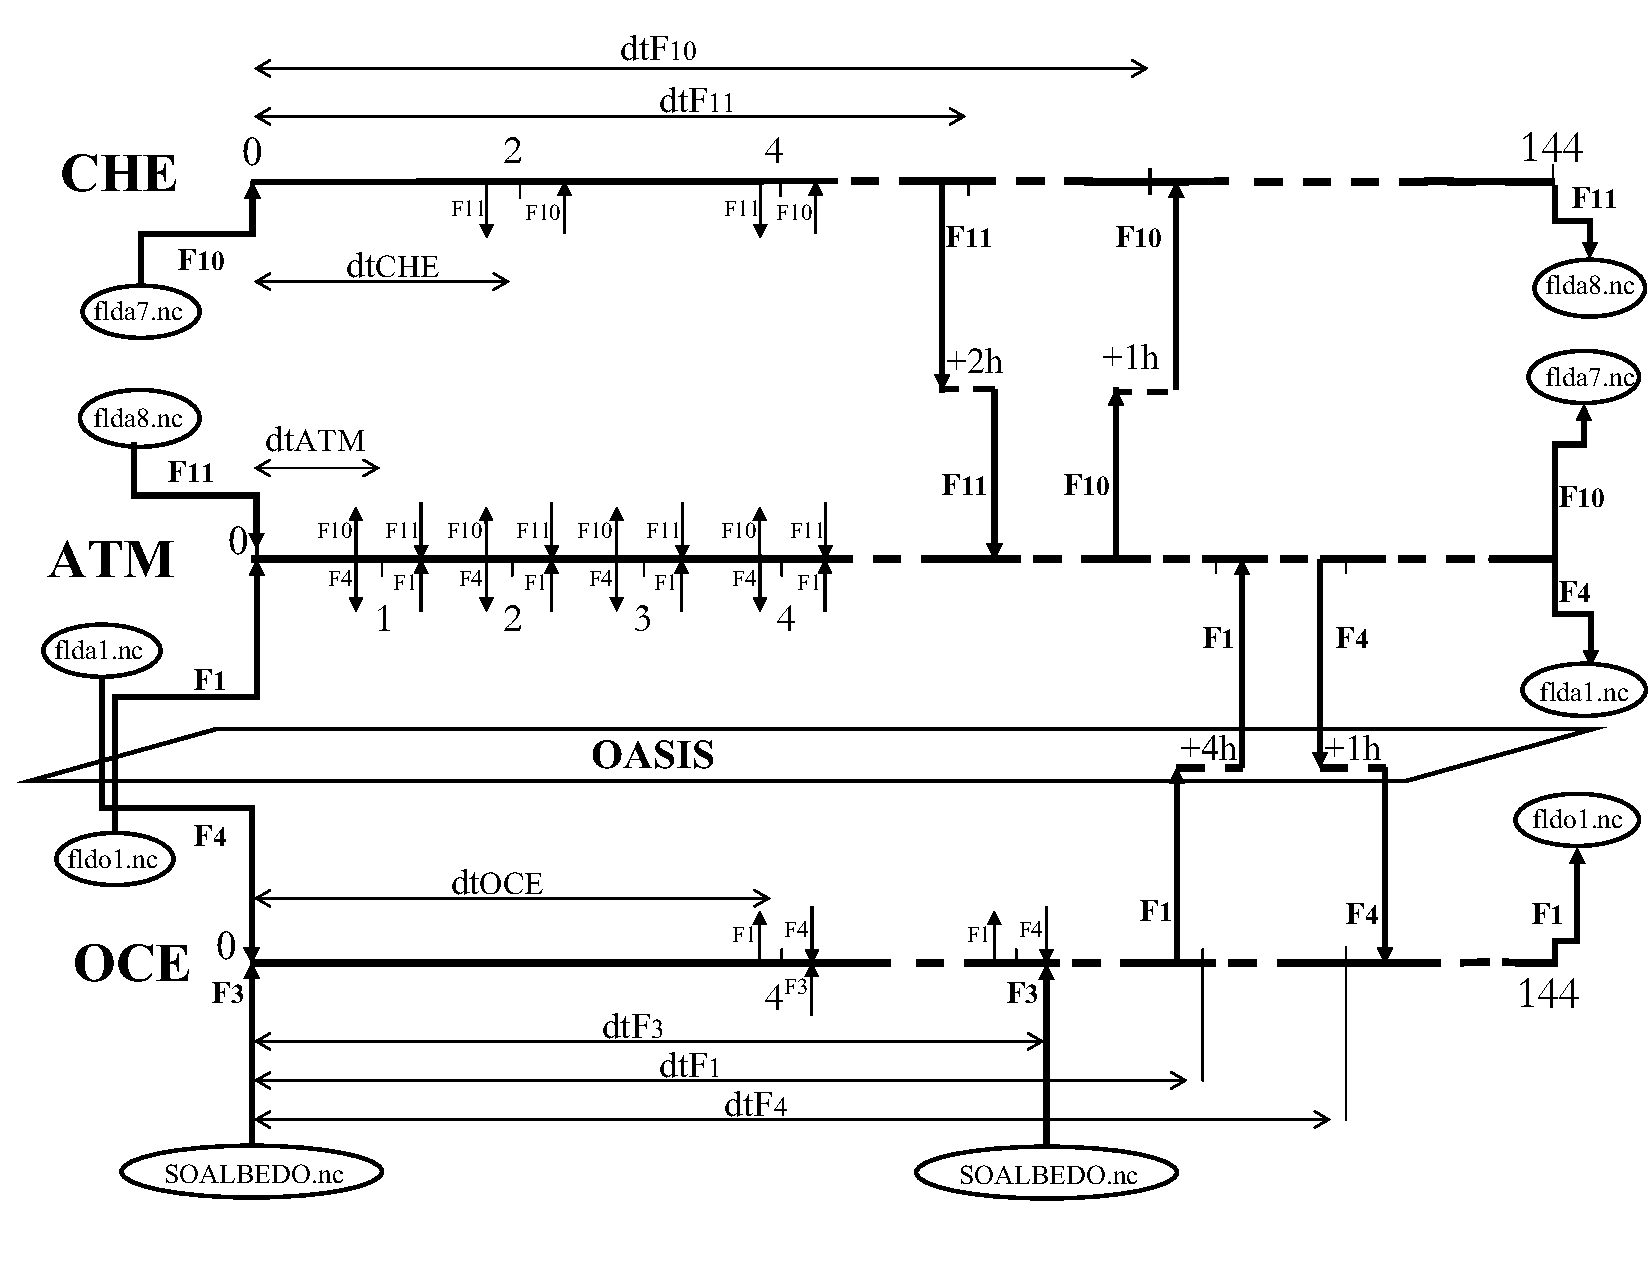
\includegraphics[scale=0.57]{figures/coupling_algo4}
%\includegraphics[scale=0.8]{figures/coupling_algo4.eps}
\caption{Exchange algorithm between the 3 TOYOASIS3 component models for
  fields $Field_1$, $Field_3$,
$Field_4$, $Field_{10}$, and $Field_{11}$. }
\label{fig:toyoasis3couplingalgo}
\end{figure}



\subsection{Compiling and Running TOYOASIS3}
\label{subsec_running_toyoasis3}

The TOYOASIS3 compiling and running environment is available in {\tt
  oasis3/examples/toyoasis3}.  

Subdirectory {\tt /data} contains auxiliary grid data files (see
\ref{subsec_griddata}) and coupling restart files (see
\ref{subsec_restartdata}). Subdirectory {\tt /input} contains the file
{\tt cf\_name\_table.txt} (see \ref{subsec_cfnametable}) the
configuration file (see chapter \ref{sec_namcouple}) used in the
classic (not parallel) mode, {\it namcouple}, and the
configuration files used in the IPSL parallel mode, 
{\it namcouple\_0} and {\it namcouple\_1}.

To run TOYOASIS3, first compile OASIS3 and the 3 TOYOASIS3 component
models (see section \ref{subsec_compile}). 
Go in directory {\tt oasis3/examples/toyoasis3/src} and type
{\tt make}.  This will automatically compile OASIS main executable and
PSMILe library, if not done before hand, and the three component
models {\tt atmoa3.x}, {\tt cheoa3.x} and {\tt oceoa3.x}, using the
header file specified in {\tt oasis3/util/make\_dir} \newline {\tt /make.inc}.

The next step is to adapt the ``User's section'' of the running script
{\tt run\_toyoasis3} in subdirectory {\tt /script} and to launch it.
The script {\tt run\_toyoasis3} supports Linux PC, NEC SX, IBM
Power4, CRAYX1, CRAYXD1 and CRAYXT platforms (see {\tt arch}
variable). If your platform is not supported, the script will
have to be adapted.

%Different modes can be tested. 
%\begin{itemize}
%\item To run in the classic (not parallel) mode, compile
%  without the CPP key {\tt use\_oasis\_para} or {\tt
%    use\_oasis\_cmcc\_para}, and set {\tt ipsl\_comp\_para=0} and {\tt
%    cmcc\_comp\_para=0} in the running script. One can now choose
%  between running atmoa3 and cheoa3 toy models on one process only
%  ({\tt nproc\_atmche=1} and {\tt ncpl\_atmche=1}) or on 3 processes
%  each ({\tt nproc\_atmche=3} and {\tt ncpl\_atmche=3}). The results
%  for the first and second cases are respectively available in {\tt
%    oasis3/examples/toyoasis3/outdata/results\_mono\_111} and \break
%  {\tt oasis3/examples/toyoasis3/outdata/results\_mono\_313} 
%  (XXX this last directory is not updated yet).
%
% Atmoa3 can run on 1 or 3 processes,
%depending on the value of the variable {\tt nproc\_atmche} in script {\tt run\_toyoasis3}. 
%When running on 3 processes, atmoa3 can either exchange coupling data
%through its 3 processes ( {\tt ncpl\_atmche = 3} in {\tt run\_toyoasis3} and  {\tt il\_nbcplproc = 3} in atmoa3.F90) or only 
%through the master process ( {\tt ncpl\_atmche = 1} in {\tt run\_toyoasis3} and  {\tt il\_nbcplproc = 1} in atmoa3.F90). 
%When atmoa3 runs or exchanges data with only one process, it defines
%one Serial partition containing the 96X48 grid points. If it runs and exchanges
%coupling data with 3 processes, its decomposition
%depends on the {\tt cdec} parameter hard coded in routine {\tt decomp\_def.F90}.
%When {\tt cdec = APPLE}, each of the 3 atmoa3 processes calls the PSMILe
%prism\_def\_partition routine to define 1 segment of an APPLE
%decomposition (1536 grid points per segment). If {\tt cdec = BOX}, each process will define 1
%`box' of a BOX decomposition and will treat a box of
%32X48 points.
%If the user hardcodes {\tt cdec = ORANGE}, each process will define a
%partition of two segments of 768 points distant of 1536 points.
%
%\item Setting {\tt gridswr=1} in the script {\tt run\_toyoasis3} will make
%the toy models to create the grid data files {\em grids.nc, masks.nc}
%and {\em areas.nc} and to write their grids, corners, areas and masks
%in these files using the {\tt prism\_write\_grid}, {\tt
%  prism\_write\_corner}, {\tt prism\_write\_mask} and {\tt
%  prism\_write\_area} routines (see \ref{subsubsec_griddef}). This
%does not change the results.
%
%\item To run in IPSL parallelisation mode, set {\tt ipsl\_comp\_para=1}. In this case,
%make sure that the CPP key {\tt use\_oasis\_para} was used for
%compilation. The script will launch OASIS3 on two processes treating
%each one a subset of the coupling fields; the first OASIS3 process
%will treat the coupling fields listed in {\it namcouple\_0} while the
%second will treat the coupling fields listed in {\it namcouple\_1}.
%For more details in the IPSL parallelisation mode, see section
%\ref{sec_ipslpara_mode}.  The results one should get with {\tt
%  ipsl\_comp\_para=1} (in the case the atmoa3 and cheoa3 toy models run on
%one process only) are available in {\tt
%  oasis3/examples/toyoasis3/outdata/results\_para}. (XXX This last directory is not updated yet XXX).
%
%\item To run in CMCC parallelisation mode, set {\tt
%    cmcc\_comp\_para=1}. In this case, make sure that the CPP key {\tt
%    use\_oasis\_cmcc\_para} was used for compilation.  For more
%  details in the CMCC parallelisation mode, see section
%  \ref{sec_cmccpara_mode}. The results one should get with {\tt
%    cmcc\_comp\_para=1} are available in ... (XXX to be completed)
%
%\end{itemize}
%
%\section{Running OASIS3 in interpolator-only mode}
%
%OASIS3 can be used in an interpolator-only mode, in which case it
%transforms fields without running any model (see section
%\ref{subsec_interpolator}). Two test-cases are provided with OASIS3 to
%illustrate its uses in this mode, the ``testinterp'' test-case (see
%section \ref{subsec_running_testinterp}) and the ``testNONE''
%test-case (see section \ref{subsec_running_testnone}). 
%
%\subsection{The ``testinterp'' test-case}
%\label{subsec_running_testinterp}
%
%The ``testinterp'' test-case can be run to test the interpolation of
%different source fields corresponding to analytical functions 
%and to evaluate the error between the
%interpolated fields and the same analytical functions calculated on the
%different target grids.
%
%All files needed to run this test-case can be found in
%{\tt oasis3/examples/testinterp/input} and {\tt oasis3/examples/testinterp/restart}.
%
%To run ``testinterp'', OASIS3 first has to be compiled (see section \ref{sec_notSCE}) in
%interpolator-only mode NONE, i.e. by putting 
%{\tt CHAN = NONE} in the TopMakefileOasis3 header file. Then
%the programs that will calculate the interpolation error, i.e. {\tt
%  gen\_error.f90} and {\tt gen\_error\_vector.f90} (for vector
%fields) in directory {\tt oasis3/examples/testinterp/error} have to
%be compiled (see script {\tt sc\_comp\_error}).
%
%Then, one has to adapt and execute the running script {\tt
%  oasis3/examples/testinterp/\break sc\_run\_testinterp}.
%With {\tt TIME=ONE}, the configuration file {\tt
%  oasis3/examples/testinterp/\break input/namcouple\_ONE}, the input files
%{\tt flda1.nc, flda2.nc, flda3.nc, fldb1.nc,} \newline {\tt fldo1.nc}
%and {\tt fldz1.nc} from {\tt oasis3/examples/testinterp/restart} and the
%input files {\tt aaIin.nc} and {\tt caJin.nc} from {\tt
%  oasis3/examples/testinterp/restart/vector} are used.  This example also
%shows one vector interpolation (field components {\tt a\_at42\_I} and
%{\tt c\_at42\_J}).  The test-case automatically writes the error
%fields in {\tt error\_*.nc} files and error statistics in {\tt log\_*}
%files.
%
%To run the example into which OASIS3 interpolates many time
%occurrences from one input file, put {\tt TIME=MANY} in {\tt
%  sc\_run\_testinterp}.  The configuration file {\tt
%  oasis3/examples/testinterp/\break input/namcouple\_MANY} and the input
%file {\tt fldin.nc} in {\tt oasis3/examples/testinterp/\break restart} are then
%used.
%
%The results obtained after running the testinterp test-case should
%match the ones in {\tt oasis3/examples/\break testinterp/outdata}.
%(XXX this directory is not updated yet).
%
%\subsection{The ``testNONE'' test-case}
%\label{subsec_running_testnone}
%
%All files to run the ``testNONE'' test-case can be found in {\tt
%  oasis3/examples/testNONE}. This test-case provides a flexible
%environnement to test the interpolation specified in the {\tt
%  INPUT/namcouple} configuration file from a source grid to a target
%grid, both grids being defined in regular OASIS3 grid data files {\it
%  grids.nc}, {\it masks.nc}, {\it areas.nc} (see section
%\ref{subsec_griddata}). 
%
%To run ``testNONE'', OASIS3 first has to be compiled (see section \ref{sec_notSCE}) in
%interpolator-only mode NONE, i.e. by putting 
%{\tt CHAN = NONE} in the TopMakefileOasis3 header file. 
%The user then has to adapt the ``User specifications''
%part of the running script {\tt sc\_run\_NONE}. In particular, he has
%to specify:
%\begin{itemize}
%\item {\tt DIRWORK} : the directory where to run the test-case
%\item {\tt BINDIR} : the directory containing OASIS3 executable
%\item {\tt SRCROOT} : the source of the {\tt oasis3} directory
%\item {\tt ARCH} : the platform onto which the test-case will run
%\item {\tt DIR\_GRD} : the directory for the grid data files
%\item {\tt DIR\_INP} : the directory for the {\it namcouple} and {\tt cf\_name\_table.txt} files  
%\item {\tt SRC\_GRID} and {\tt TGT\_GRID} : the source
%and target grid prefixes in the {\it namcouple} and in the grid data
%files (see section \ref{subsubsec_secondEXPORTED}), 
%\item {\tt FLD\_NBR} : the number of the analytic function chosen, 
%\item {\tt MASKERROR} : whether or not the error on the target grid will be
%calculated on all points ({\tt MASKERROR=NOT}) or only on non masked
%points ({\tt MASKERROR=YES}).
%\end{itemize}
%
%When launched, the running script {\tt sc\_run\_NONE}:
%\begin{itemize}
%\item creates a working directory
%\item compiles and runs the program {\tt
%    PROG/create\_inputfield.f90} that creates an input field using the
%  chosen analytical function on the specified source grid in file
%  {\tt fldin.nc}
%\item copy all required input and data file to the working directory 
%\item run OASIS3 that interpolates the analytical field from {\tt
%    fldin.nc} with the interpolation specified in the {\it namcouple}
%\item compile and run the program {\tt PROG/create\_errorfield.f90}
%  that calculates the error between the resulting interpolated field
%  and the field defined by the chosen analytical function on the
%  specified target grid, and writes it to the file {\tt error.nc}
%\end{itemize}
%
\section{Known problems when compiling or running OASIS3 on specific platforms}

\begin{itemize}
\item  Notes on porting to BlueGeneL (XXX to be detailed):
% OASIS sur le BlueGene:
% voir le message a Honore Tapamo du 12/03/2008 dans oasis4_0/oasis4\_0\_uti
% et a Metafor le 02/19/2009 dans oasis4\_0/oasis4\_0\_uti

% On the Blue Gene L, it takes some time when launching the coupled model, 
% but then it works fine without significant loss of performance.
% XXXXX

\item  Notes on porting to BlueGeneP (XXX to be detailed):
% Plusieurs difficultés:
% 1) Il faut qu'OASIS3 utilise au moins un ensemble de 64 processeurs (1
%    pset); il faut donc utiliser OASIS3 pseudo-parallel et le modifier
%    de facon a ce que les processus OASIS3 inutiles traitent 0 champs
%    (cf les modifs d'Arnaud)
% 2) Il est impossible sur cette machine de s'assurer que tous les
%    processus OASIS3 sont contigus et commencent avec rank=0; donc il
%    faudrait modifier OASIS3 pour enlever cette restriction (en MPI1)
% Donc autant mettre l'effort sur le portage d'OASIS4. XXXX

%
%\item Tests have detected a bug with the {\tt transfer} function of
%   the Portland Group Fortran 90 compiler versions 5.2.4, 6.1.3 or 7.0
%   in 64 bit mode. The {\tt transfer} function is used in {\tt
%     prism/src/lib/mpp\_io/src/mpp\_io\_mod\_oa.F90} and {\tt
%     mpp\_mod\_oa.F90} .
%
\end{itemize}
